%package list
\documentclass{article}
\usepackage[top=3cm, bottom=3cm, outer=3cm, inner=3cm]{geometry}
\usepackage{multicol}
\usepackage{graphicx}
\usepackage{url}
%\usepackage{cite}
\usepackage{hyperref}
\usepackage{array}
%\usepackage{multicol}
\newcolumntype{x}[1]{>{\centering\arraybackslash\hspace{0pt}}p{#1}}
\usepackage{natbib}
\usepackage{pdfpages}
\usepackage{multirow}
\usepackage[normalem]{ulem}
\useunder{\uline}{\ul}{}
\usepackage{svg}
\usepackage{xcolor}
\usepackage{listings}
\lstdefinestyle{ascii-tree}{
    literate={├}{|}1 {─}{--}1 {└}{+}1 
  }
\lstset{basicstyle=\ttfamily,
  showstringspaces=false,
  commentstyle=\color{red},
  keywordstyle=\color{blue}
}
%\usepackage{booktabs}
\usepackage{caption}
\usepackage{subcaption}
\usepackage{float}
\usepackage{array}

\newcolumntype{M}[1]{>{\centering\arraybackslash}m{#1}}
\newcolumntype{N}{@{}m{0pt}@{}}


%%%%%%%%%%%%%%%%%%%%%%%%%%%%%%%%%%%%%%%%%%%%%%%%%%%%%%%%%%%%%%%%%%%%%%%%%%%%
%%%%%%%%%%%%%%%%%%%%%%%%%%%%%%%%%%%%%%%%%%%%%%%%%%%%%%%%%%%%%%%%%%%%%%%%%%%%
\newcommand{\itemEmail}{schirinosne@unsa.edu.pe}
\newcommand{\itemStudent}{Sebastian Arley Chirinos Negrón
Rodrigo Estefano Viza Cuti
Daniel Enrique Marrón Carcausto
Diego Renato Llerena Tellez}
\newcommand{\itemCourse}{Programación Web 2}
\newcommand{\itemCourseCode}{1702122}
\newcommand{\itemSemester}{I}
\newcommand{\itemUniversity}{Universidad Nacional de San Agustín de Arequipa}
\newcommand{\itemFaculty}{Facultad de Ingeniería de Producción y Servicios}
\newcommand{\itemDepartment}{Departamento Académico de Ingeniería de Sistemas e Informática}
\newcommand{\itemSchool}{Escuela Profesional de Ingeniería de Sistemas}
\newcommand{\itemAcademic}{2023 - A}
\newcommand{\itemInput}{Del 31 Julio 2023}
\newcommand{\itemOutput}{Al 07 Agosto 2023}
\newcommand{\itemPracticeNumber}{09}
\newcommand{\itemTheme}{Proyecto Final}
%%%%%%%%%%%%%%%%%%%%%%%%%%%%%%%%%%%%%%%%%%%%%%%%%%%%%%%%%%%%%%%%%%%%%%%%%%%%
%%%%%%%%%%%%%%%%%%%%%%%%%%%%%%%%%%%%%%%%%%%%%%%%%%%%%%%%%%%%%%%%%%%%%%%%%%%%

\usepackage[english,spanish]{babel}
\usepackage[utf8]{inputenc}
\AtBeginDocument{\selectlanguage{spanish}}
\renewcommand{\figurename}{Figura}
\renewcommand{\refname}{Referencias}
\renewcommand{\tablename}{Tabla} %esto no funciona cuando se usa babel
\AtBeginDocument{%
	\renewcommand\tablename{Tabla}
}

\usepackage{fancyhdr}
\pagestyle{fancy}
\fancyhf{}
\setlength{\headheight}{45pt}
\renewcommand{\headrulewidth}{1pt}
\renewcommand{\footrulewidth}{1pt}
\fancyhead[L]{\raisebox{-0.2\height}{
\includegraphics[width=3cm]{img/logo_episunsa.png}}}
\fancyhead[C]{\fontsize{7}{7}\selectfont	\itemUniversity \\ \itemFaculty \\ \itemDepartment \\ \itemSchool \\ \textbf{\itemCourse}}
\fancyhead[R]{\raisebox{-0.2\height}{
\includegraphics[width=1.2cm]{img/logo_abet}}}
\fancyfoot[L]{Chirinos, Viza, Carcausto, Llerena}
\fancyfoot[C]{\itemCourse}
\fancyfoot[R]{Página \thepage}

% para el codigo fuente
\usepackage{listings}
\usepackage{color, colortbl}
\definecolor{dkgreen}{rgb}{0,0.6,0}
\definecolor{gray}{rgb}{0.5,0.5,0.5}
\definecolor{mauve}{rgb}{0.58,0,0.82}
\definecolor{codebackground}{rgb}{0.95, 0.95, 0.92}
\definecolor{tablebackground}{rgb}{0.8, 0, 0}

\lstset{frame=tb,
	language=bash,
	aboveskip=3mm,
	belowskip=3mm,
	showstringspaces=false,
	columns=flexible,
	basicstyle={\small\ttfamily},
	numbers=none,
	numberstyle=\tiny\color{gray},
	keywordstyle=\color{blue},
	commentstyle=\color{dkgreen},
	stringstyle=\color{mauve},
	breaklines=true,
	breakatwhitespace=true,
	tabsize=3,
	backgroundcolor= \color{codebackground},
}

\begin{document}

	\vspace*{10px}

	\begin{center}	
		\fontsize{17}{17} \textbf{ Informe de Laboratorio \itemPracticeNumber}
	\end{center}
	\centerline{\textbf{\Large Tema: \itemTheme}}
	%\vspace*{0.5cm}	

	\begin{flushright}
		\begin{tabular}{|M{2.5cm}|N|}
			\hline 
			\rowcolor{tablebackground}
			\color{white} \textbf{Nota}  \\
			\hline 
			     \\[30pt]
			\hline 			
		\end{tabular}
	\end{flushright}	

	\begin{table}[H]
		\begin{tabular}{|x{4.7cm}|x{4.8cm}|x{4.8cm}|}
			\hline 
			\rowcolor{tablebackground}
			\color{white} \textbf{Estudiante} & \color{white}\textbf{Escuela}  & \color{white}\textbf{Asignatura}   \\
			\hline 
			{\itemStudent \par \itemEmail} & \itemSchool & {\itemCourse \par Semestre: \itemSemester \par Código: \itemCourseCode}     \\
			\hline 			
		\end{tabular}
	\end{table}		

	\begin{table}[H]
		\begin{tabular}{|x{4.7cm}|x{4.8cm}|x{4.8cm}|}
			\hline 
			\rowcolor{tablebackground}
			\color{white}\textbf{Laboratorio} & \color{white}\textbf{Tema}  & \color{white}\textbf{Duración}   \\
			\hline 
			\itemPracticeNumber & \itemTheme & 04 horas   \\
			\hline 
		\end{tabular}
	\end{table}

	\begin{table}[H]
		\begin{tabular}{|x{4.7cm}|x{4.8cm}|x{4.8cm}|}
			\hline 
			\rowcolor{tablebackground}
			\color{white}\textbf{Semestre académico} & \color{white}\textbf{Fecha de inicio}  & \color{white}\textbf{Fecha de entrega}   \\
			\hline 
			\itemAcademic & \itemInput &  \itemOutput  \\
			\hline 
		\end{tabular}
	\end{table}


	\section{Equipos, materiales y temas utilizados}
\begin{itemize}
    \item Programar usando Python.
    \item Utilización del framework Django para desarrollo web.
    \item Implementación de plantillas Django para la construcción de interfaces de usuario.
    \item Uso del Django Rest Framework para crear APIs RESTful.
    \item Integración de JavaScript para mejorar la interactividad en el frontend.
    \item Desarrollo de páginas web con HTML y estilización con CSS.
    \item Empleo de AJAX para realizar peticiones asíncronas en el frontend.
    \item Consumo de APIs externas, como la API de Google, para la obtención de datos.
    \item Aplicación de principios de programación orientada a objetos en el diseño del proyecto.
    \item Separación de intereses en clases: el modelo de datos y su representación visual.
    \item Utilización de listas y ciclos en el manejo y procesamiento de datos.
    \item Exploración de conceptos de programación funcional en el desarrollo del proyecto.
\end{itemize}

	\section{URL de Repositorio Github}
	\begin{itemize}
		\item URL del Repositorio GitHub para clonar o recuperar.
		\item \url{https://github.com/imlosing07/pw2-lab-D-23a.git}
	\end{itemize}

	\section{Actividades con el repositorio GitHub}

	\subsection{Creacion de de login y register}
	\subsection{forms.py}
	Este es un script de Python que define dos clases: \texttt{SignUpForm} y \texttt{LogInForm}. Ambas clases son subclases de formularios de Django, que se utilizan para manejar la entrada del usuario en aplicaciones web. La clase \texttt{SignUpForm} es una subclase de \texttt{UserCreationForm}, que es un formulario incorporado en Django para crear nuevos usuarios. La clase \texttt{LogInForm} es una subclase de \texttt{AuthenticationForm}, que es un formulario incorporado en Django para autenticar a usuarios existentes.

La clase \texttt{SignUpForm} tiene un método \texttt{\_\_init\_\_} que personaliza los campos del formulario para el nombre de usuario, password1 y password2. El método actualiza los atributos del widget para estos campos para agregar clases CSS, establecer el tipo de entrada y agregar texto de marcador de posición. La clase también define dos campos adicionales del formulario: \texttt{username} y \texttt{email}. La clase \texttt{Meta} dentro de la clase \texttt{SignUpForm} especifica que el formulario debe usar el modelo incorporado en Django \texttt{User} e incluir los campos para el nombre de usuario, password1 y password2.

La clase \texttt{LogInForm} también tiene un método \texttt{\_\_init\_\_} que personaliza los campos del formulario para el nombre de usuario y la contraseña. Al igual que el \texttt{SignUpForm}, este método actualiza los atributos del widget para estos campos. La clase también define un campo adicional del formulario para el nombre de usuario. La clase \texttt{Meta} dentro del \texttt{LogInForm} especifica que el formulario debe usar el modelo incorporado en Django \texttt{User} e incluir los campos para el nombre de usuario y la contraseña.



	\lstinputlisting[language=Python, caption={forms.py},numbers=left,]{src/forms.py}	

	\subsection{Models.py}
	\begin{itemize}
		\item El modelo \texttt{Category} representa una categoría de productos en la tienda. Tiene campos como \texttt{nombre}, \texttt{id\_categoria}, \texttt{created\_date}, \texttt{modify\_date}, \texttt{status} y \texttt{user\_id}.
		\item El modelo \texttt{Product} representa un producto en la tienda. Tiene campos como \texttt{name}, \texttt{description}, \texttt{price}, \texttt{stock}, \texttt{image\_url}, \texttt{category}, \texttt{created\_date}, \texttt{modify\_date}, \texttt{status} y \texttt{user\_id}.
		\item El modelo \texttt{Customer} representa a un cliente en la tienda. Tiene campos como \texttt{user}, \texttt{shipping\_address}, \texttt{created\_date}, \texttt{modify\_date}, \texttt{status} y \texttt{user\_id}.
		\item El modelo \texttt{Order} representa a un pedido en la tienda. Tiene campos como \texttt{customer}, \texttt{items}, \texttt{total\_amount}, \texttt{status}, \texttt{created\_date}, \texttt{modify\_date} y \texttt{user\_id}.
	\end{itemize}
	
	


	\lstinputlisting[language=Python, caption={models.py},numbers=left,]{src/models.py}	

	\begin{itemize}	
		\item UML de los modelos:
	\end{itemize}	

	\begin{figure}[H]
		\centering
		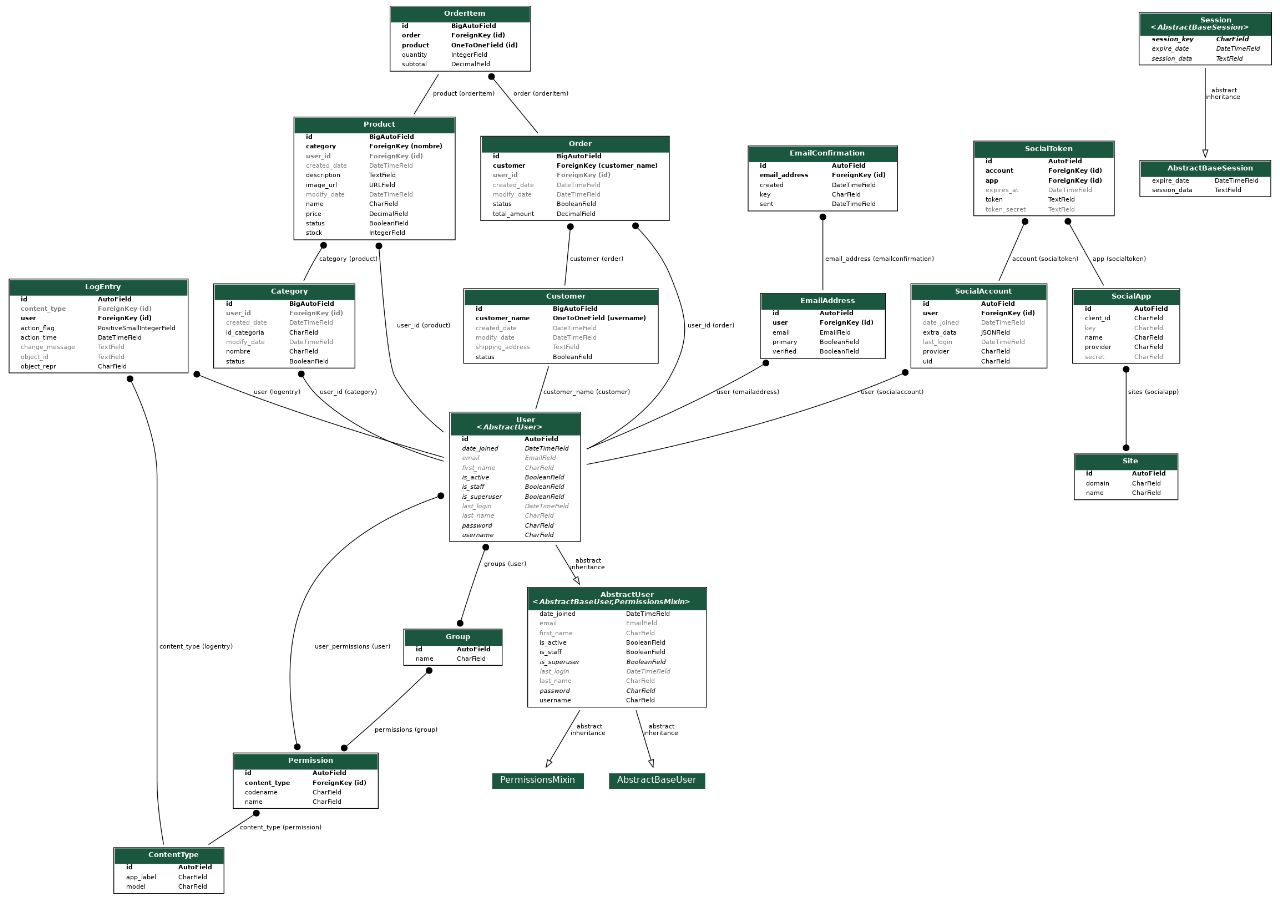
\includegraphics[width=1\textwidth,keepaspectratio]{img/UML.jpeg}
		%\includesvg{img/automata.svg}
		%\label{img:mot2}
		%\caption{Product backlog.}
	\end{figure}


	\subsection{views.py}
	\begin{itemize}	
		
			\item La vista \texttt{home} simplemente devuelve una respuesta que renderiza la plantilla \texttt{index.html}.
			\item La vista \texttt{carrito} también devuelve una respuesta que renderiza la plantilla \texttt{carrito.html}.
			\item La vista \texttt{signin} maneja el registro de nuevos usuarios en el sitio web. Si la solicitud es un método GET, la vista devuelve una respuesta que renderiza la plantilla \texttt{signin.html} con un formulario de registro. Si la solicitud es un método POST, la vista verifica si las contraseñas ingresadas coinciden y, de ser así, intenta crear un nuevo usuario con el nombre de usuario y la contraseña proporcionados. Si el usuario se crea correctamente, se inicia sesión automáticamente y se redirige a la página de inicio. Si ocurre un error al crear el usuario (por ejemplo, si el nombre de usuario ya está en uso), se devuelve una respuesta que renderiza la plantilla \texttt{signin.html} con un mensaje de error.
			\item La vista \texttt{user\_login} maneja el inicio de sesión de usuarios existentes en el sitio web. Si la solicitud es un método GET, la vista devuelve una respuesta que renderiza la plantilla \texttt{login.html} con un formulario de inicio de sesión. Si la solicitud es un método POST, la vista intenta autenticar al usuario con el nombre de usuario y la contraseña proporcionados. Si el usuario se autentica correctamente, se inicia sesión y se redirige a la página de inicio. Si ocurre un error al autenticar al usuario (por ejemplo, si el nombre de usuario o la contraseña son incorrectos), se devuelve una respuesta que renderiza la plantilla \texttt{login.html} con un mensaje de error.
			\item La vista \texttt{user\_logout} maneja el cierre de sesión de usuarios en el sitio web. Simplemente cierra la sesión del usuario actual y redirige a la página de inicio.
	\end{itemize}	

	\lstinputlisting[language=Python, caption={views.py},numbers=left,]{src/views.py}	
	
	\subsection{CAPTURAS DEL Proyecto}
	\begin{figure}[H]
		\centering
		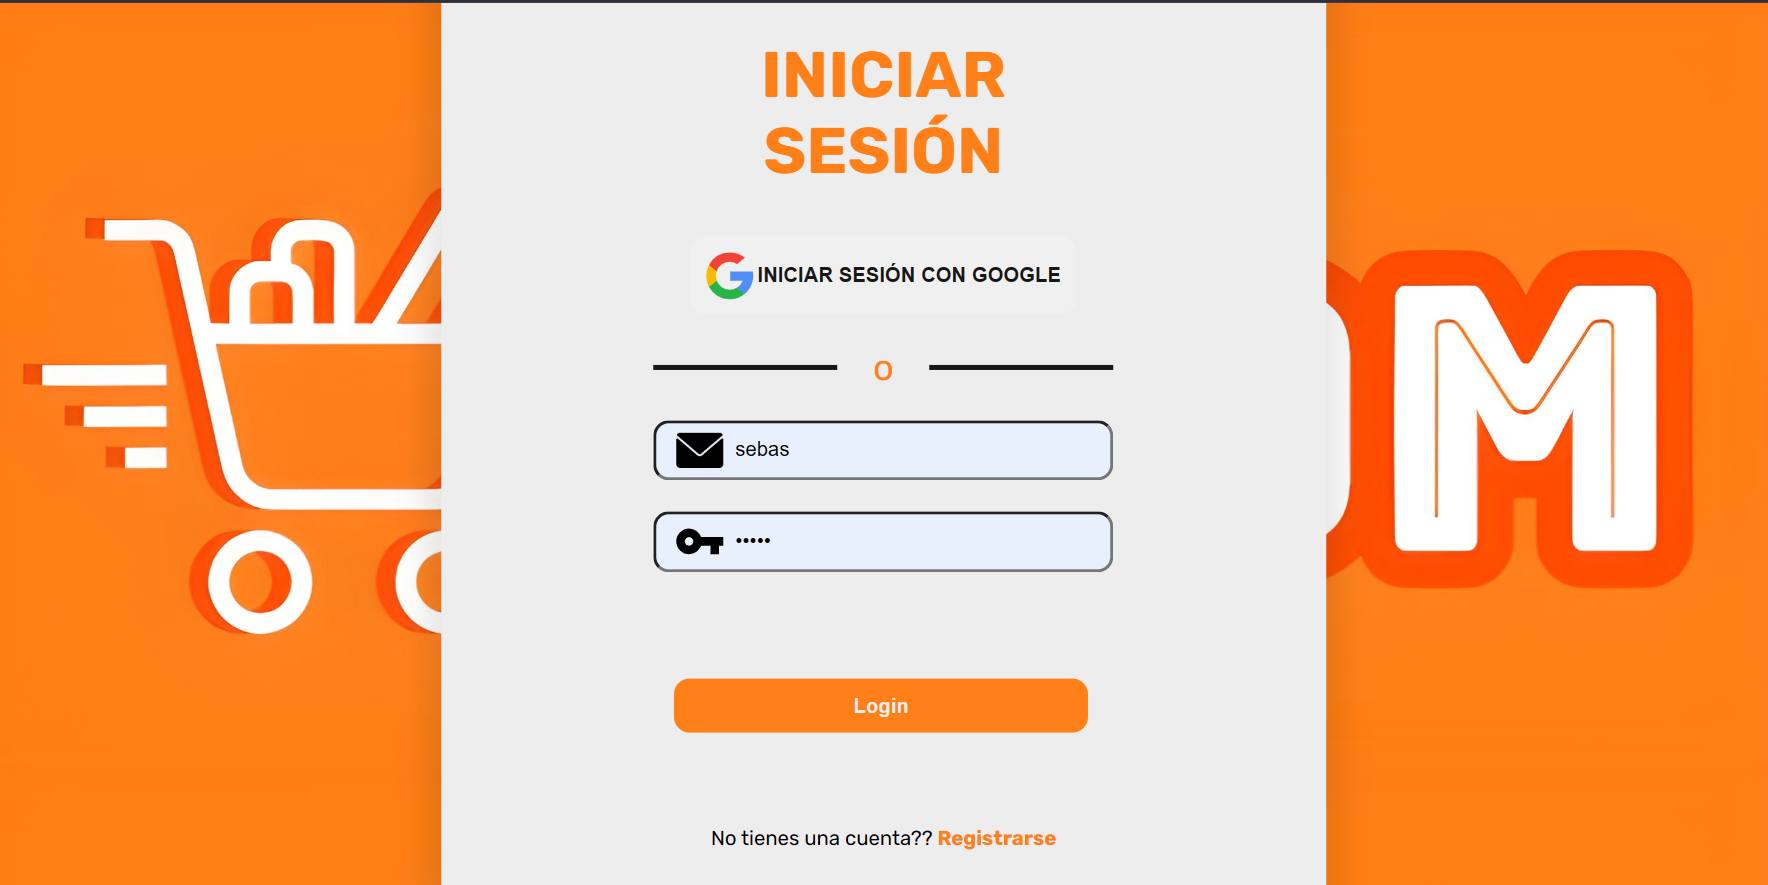
\includegraphics[width=0.6\textwidth,keepaspectratio]{img/1.png}
		%\includesvg{img/automata.svg}
		%\label{img:mot2}
		%\caption{Product backlog.}
	\end{figure}
	\begin{figure}[H]
		\centering
		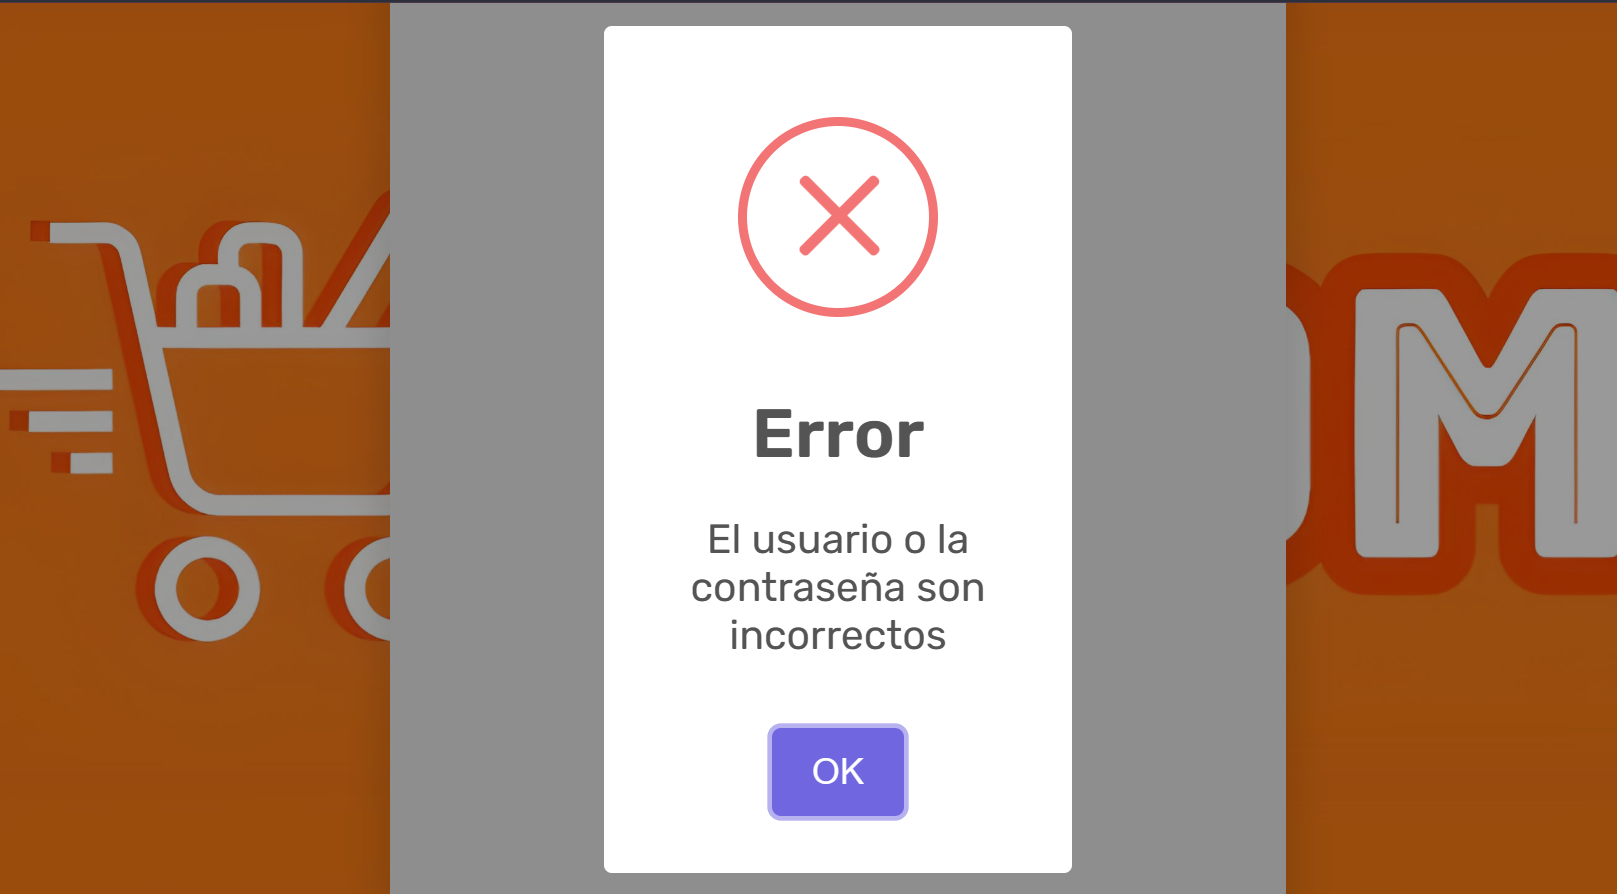
\includegraphics[width=0.6\textwidth,keepaspectratio]{img/2.png}
		%\includesvg{img/automata.svg}
		%\label{img:mot2}
		%\caption{Product backlog.}
	\end{figure}
	\begin{figure}[H]
		\centering
		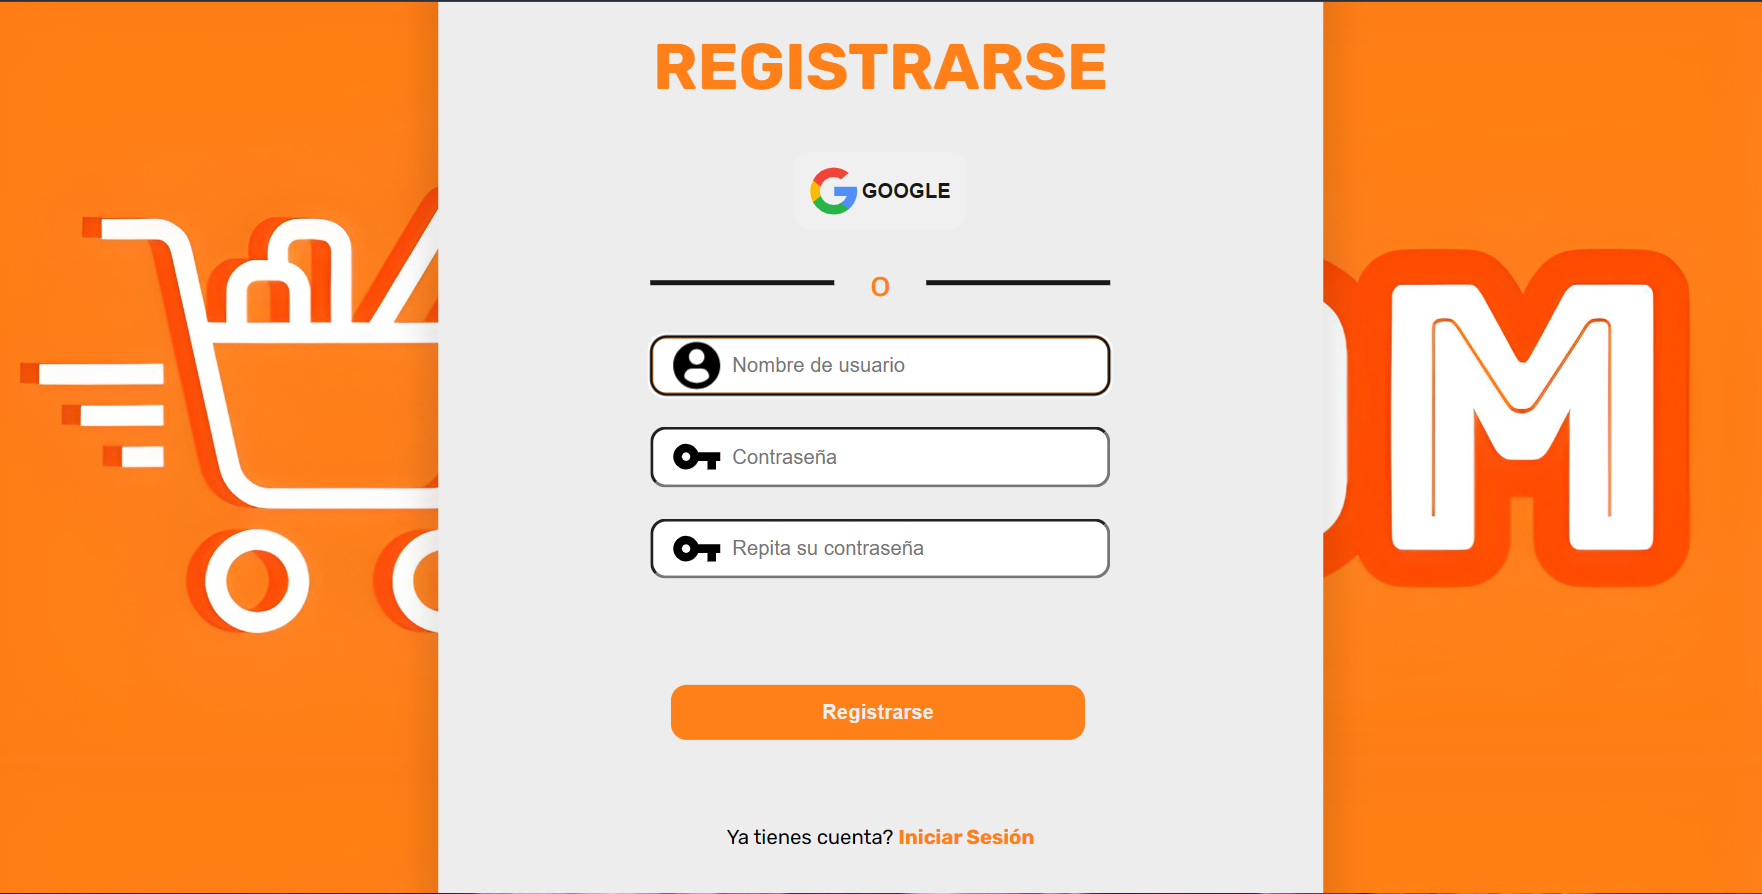
\includegraphics[width=0.6\textwidth,keepaspectratio]{img/3.png}
		%\includesvg{img/automata.svg}
		%\label{img:mot2}
		%\caption{Product backlog.}
	\end{figure}
	\begin{figure}[H]
		\centering
		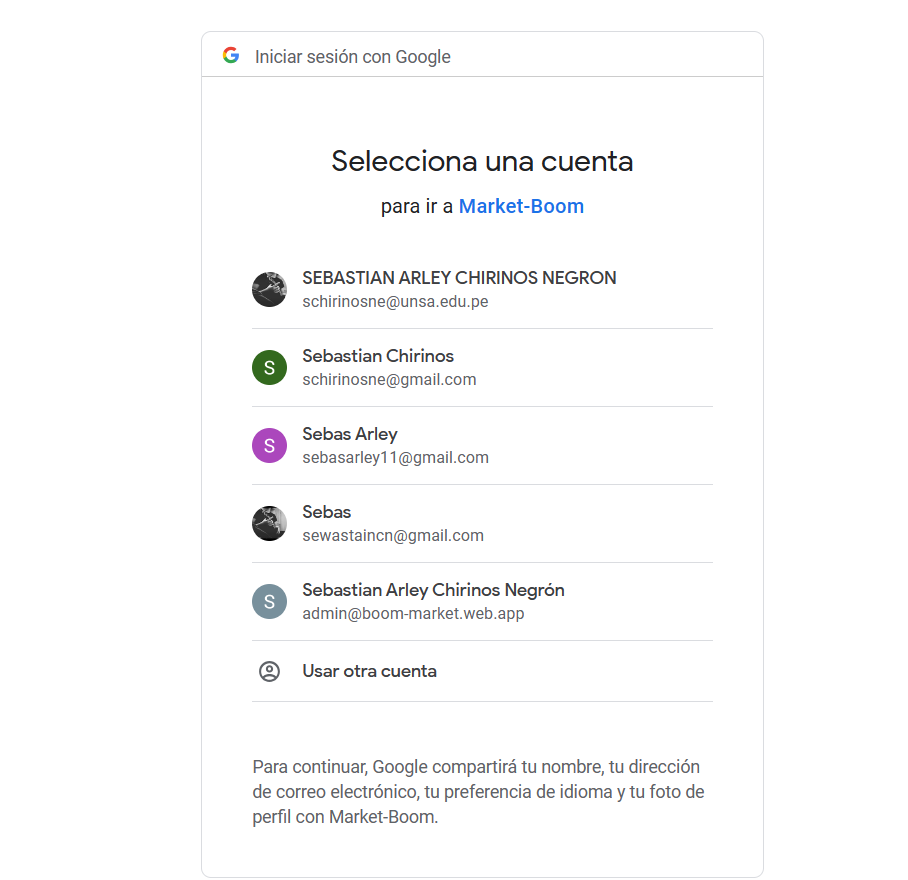
\includegraphics[width=0.6\textwidth,keepaspectratio]{img/4.png}
		%\includesvg{img/automata.svg}
		%\label{img:mot2}
		%\caption{Product backlog.}
	\end{figure}
	\begin{figure}[H]
		\centering
		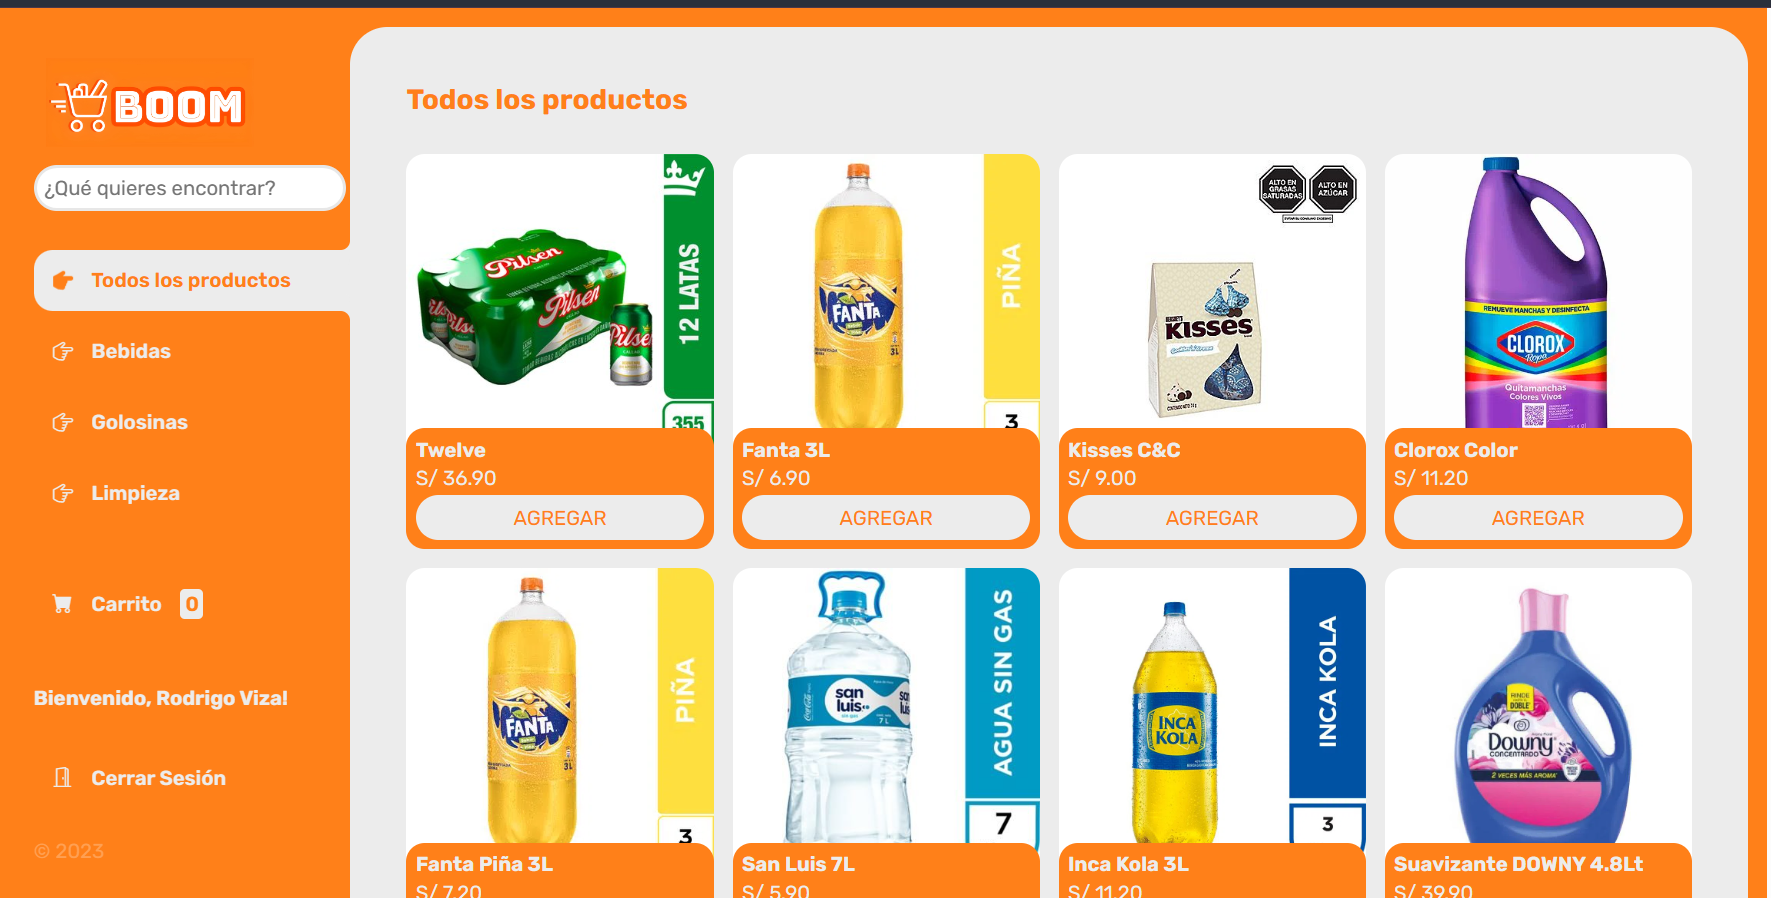
\includegraphics[width=0.6\textwidth,keepaspectratio]{img/5.png}
		%\includesvg{img/automata.svg}
		%\label{img:mot2}
		%\caption{Product backlog.}
	\end{figure}
	\begin{figure}[H]
		\centering
		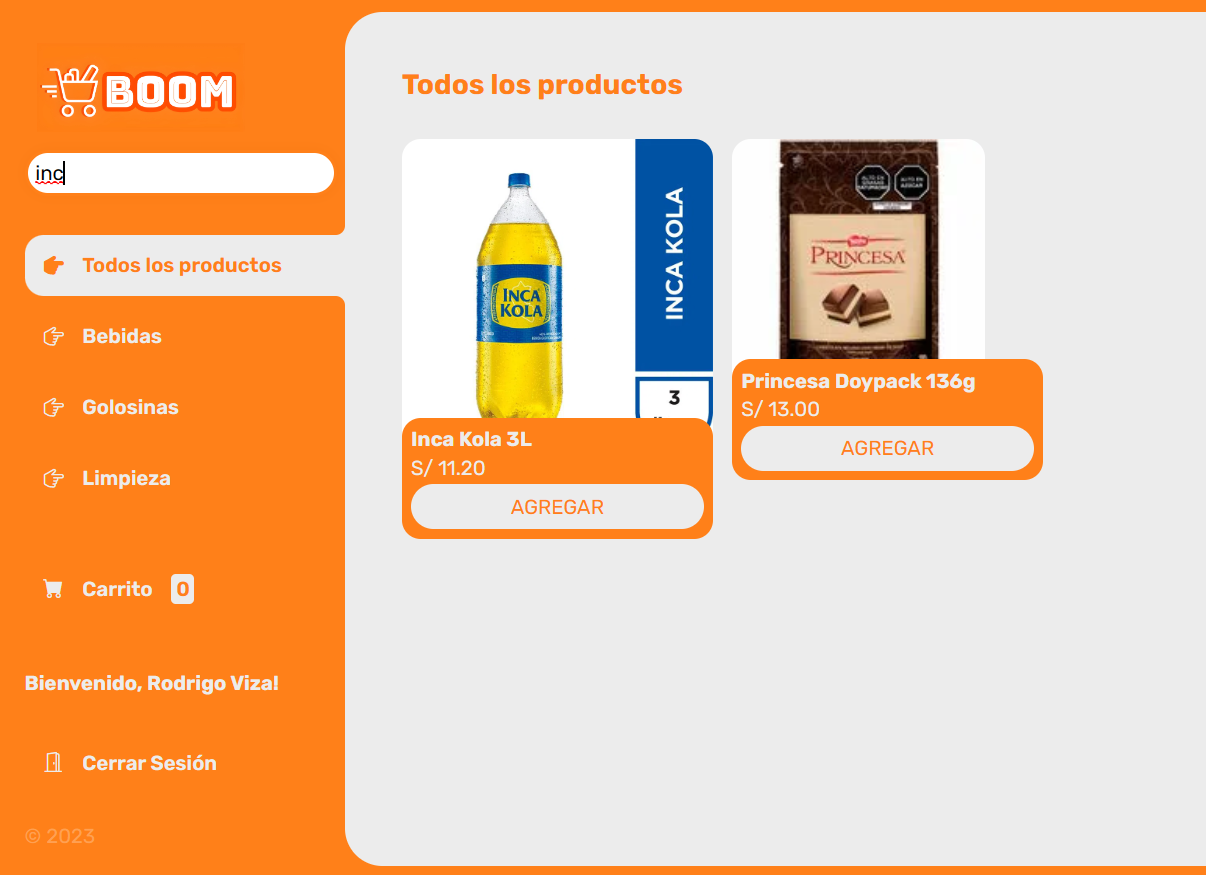
\includegraphics[width=0.6\textwidth,keepaspectratio]{img/6.png}
		%\includesvg{img/automata.svg}
		%\label{img:mot2}
		%\caption{Product backlog.}
	\end{figure}
	\begin{figure}[H]
		\centering
		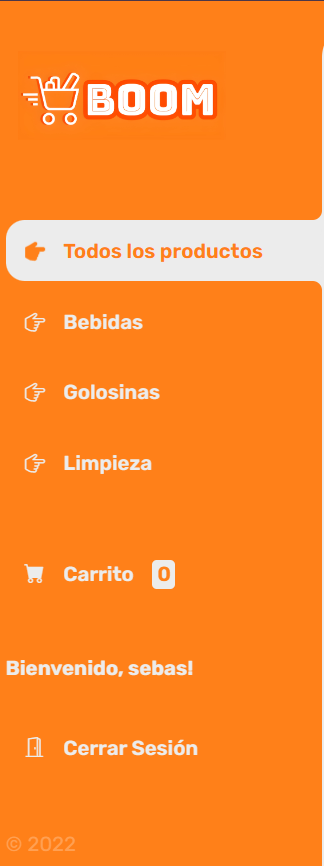
\includegraphics[width=0.6\textwidth,keepaspectratio]{img/7.png}
		%\includesvg{img/automata.svg}
		%\label{img:mot2}
		%\caption{Product backlog.}
	\end{figure}
	\begin{figure}[H]
		\centering
		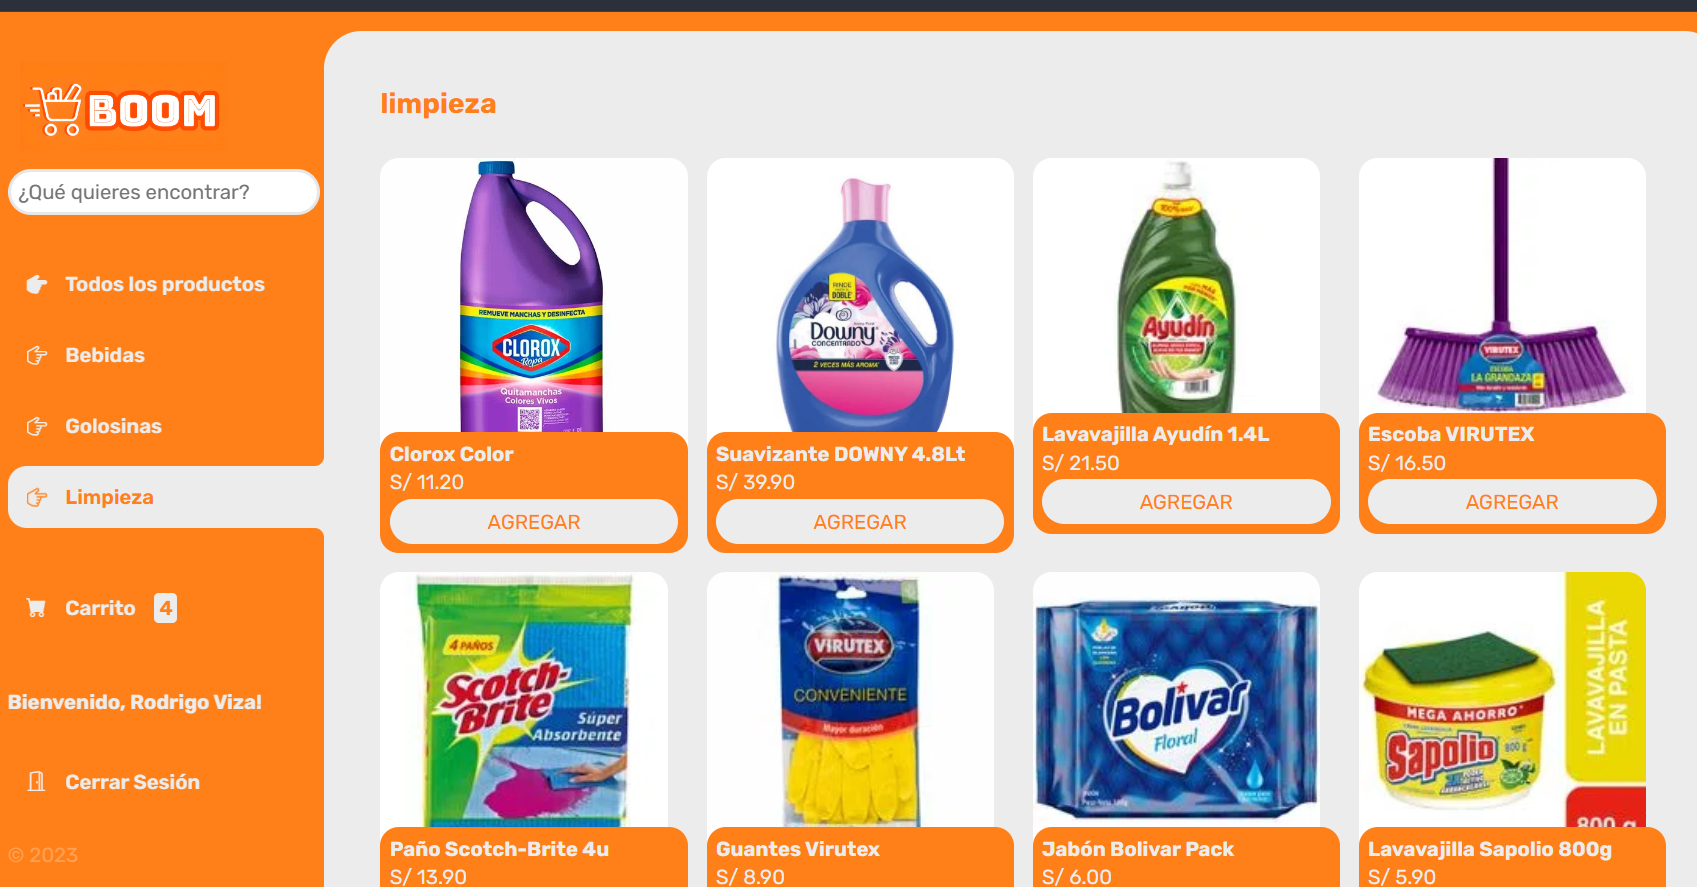
\includegraphics[width=0.6\textwidth,keepaspectratio]{img/8.png}
		%\includesvg{img/automata.svg}
		%\label{img:mot2}
		%\caption{Product backlog.}
	\end{figure}

	\begin{figure}[H]
		\centering
		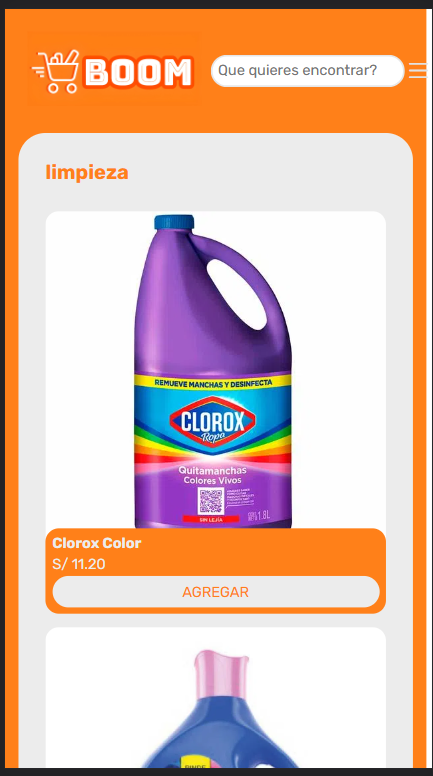
\includegraphics[width=0.6\textwidth,keepaspectratio]{img/9.png}
		%\includesvg{img/automata.svg}
		%\label{img:mot2}
		%\caption{Product backlog.}
	\end{figure}

	

	\subsection{Estructura deL Proyecto final}
	\begin{itemize}	
		\item El contenido que se entrega en este laboratorio es el siguiente:
	\end{itemize}

\begin{lstlisting}[style=ascii-tree]
ProyectoFinal/
|   .gitignore
|   Pweb02_Proyecto-Final.pdf
|   Pweb02_Proyecto-Final.tex
|
+---img
|       1.png
|       2.png
|       3.png
|       4.png
|       5.png
|       6.png
|       8.png
|       logo_abet.png
|       logo_episunsa.png
|       logo_unsa.jpg
|
\---src
        models.py
        views.py
        forms.py
        serializer.py
\end{lstlisting}    


\subsection{\textcolor{red}{Rúbrica para el contenido del Informe y demostración}}
\begin{itemize}			
	\item El alumno debe marcar o dejar en blanco en celdas de la columna \textbf{Checklist} si cumplio con el ítem correspondiente.
	\item Si un alumno supera la fecha de entrega,  su calificación será sobre la nota mínima aprobada, siempre y cuando cumpla con todos lo items.
	\item El alumno debe autocalificarse en la columna \textbf{Estudiante} de acuerdo a la siguiente tabla:

	\begin{table}[ht]
		\caption{Niveles de desempeño}
		\begin{center}
		\begin{tabular}{ccccc}
			\hline
			 & \multicolumn{4}{c}{Nivel}\\
			\cline{1-5}
			\textbf{Puntos} & Insatisfactorio 25\%& En Proceso 50\% & Satisfactorio 75\% & Sobresaliente 100\%\\
			\textbf{2.0}&0.5&1.0&1.5&2.0\\
			\textbf{4.0}&1.0&2.0&3.0&4.0\\
		\hline
		\end{tabular}
	\end{center}
\end{table}	

\end{itemize}

\begin{table}[H]
	\caption{Rúbrica para contenido del Informe y demostración}
	\setlength{\tabcolsep}{0.5em} % for the horizontal padding
	{\renewcommand{\arraystretch}{1.5}% for the vertical padding
	%\begin{center}
	\begin{tabular}{|p{2.7cm}|p{7cm}|x{1.3cm}|p{1.2cm}|p{1.5cm}|p{1.1cm}|}
		\hline
		\multicolumn{2}{|c|}{Contenido y demostración} & Puntos & Checklist & Estudiante & Profesor\\
		\hline
		\textbf{1. GitHub} & Hay enlace URL activo del directorio para el  laboratorio hacia su repositorio GitHub con código fuente terminado y fácil de revisar. &2 &X &2 & \\ 
		\hline
		\textbf{2. Commits} &  Hay capturas de pantalla de los commits más importantes con sus explicaciones detalladas. (El profesor puede preguntar para refrendar calificación). &4 & x&3 & \\ 
		\hline 
		\textbf{3. Código fuente} &  Hay porciones de código fuente importantes con numeración y explicaciones detalladas de sus funciones. &2 &X &2 & \\ 
		\hline 
		\textbf{4. Ejecución} & Se incluyen ejecuciones/pruebas del código fuente  explicadas gradualmente. &2 &X &2 & \\ 
		\hline			
		\textbf{5. Pregunta} & Se responde con completitud a la pregunta formulada en la tarea.  (El profesor puede preguntar para refrendar calificación).  &2 &X &2 & \\ 
		\hline	
		\textbf{6. Fechas} & Las fechas de modificación del código fuente estan dentro de los plazos de fecha de entrega establecidos. &2 &X &2 & \\ 
		\hline 
		\textbf{7. Ortografía} & El documento no muestra errores ortográficos. &2 &X &2 & \\ 
		\hline 
		\textbf{8. Madurez} & El Informe muestra de manera general una evolución de la madurez del código fuente,  explicaciones puntuales pero precisas y un acabado impecable.   (El profesor puede preguntar para refrendar calificación).  &4 &x &4 & \\ 
		\hline
		\multicolumn{2}{|c|}{\textbf{Total}} &20 & &19 & \\ 
		\hline
	\end{tabular}
	%\end{center}
	%\label{tab:multicol}
	}
\end{table}	

\section{Referencias}
\begin{itemize}			
	\item \url{https://www.w3schools.com/python/python_reference.asp}
	\item \url{https://docs.python.org/3/tutorial/}
\end{itemize}	

%\clearpage
%\bibliographystyle{apalike}
%\bibliographystyle{IEEEtranN}
%\bibliography{bibliography}

\end{document}